\documentclass[14pt]{extarticle}
\usepackage[T1]{fontenc}
\usepackage{tgheros}
\renewcommand{\familydefault}{\sfdefault}
\usepackage[letterpaper,left=0.75in,right=0.75in,top=0.8in,bottom=0.8in,
  headheight=16pt,headsep=16pt,footskip=28pt]{geometry}
\usepackage{tikz}
\definecolor{slotred}{RGB}{248,182,182}
\definecolor{slotblue}{RGB}{112,152,228}
\usepackage{array}
\usepackage{fancyhdr}
\pagestyle{fancy}
\fancyhf{}
\fancyhead[L]{\normalsize Week NN / Towers from either end / Grades K--1}
\fancyfoot[L]{\small Bellingham Math Circle / Week NN / NN-K-v1}
\fancyfoot[R]{\small \thepage}
\renewcommand{\headrulewidth}{0pt}
\setlength{\parindent}{0pt}
\setlength{\parskip}{5pt}
\newcounter{prob}
\newcommand{\problem}{\par\bigskip\stepcounter{prob}\noindent\textbf{Problem \theprob:} }
\newcommand{\ruledlines}[2]{\par\noindent\begin{tikzpicture}
  \foreach \k in {1,...,#1}{\draw[black!35] (0,-\k*#2) -- (\linewidth-1pt,-\k*#2);}
  \end{tikzpicture}\par}
\begin{document}

Build the towers on a strip and play with a partner. Take turns. On your
turn, take one whole tower from either end of the row. At the end, each
player snaps their cubes into one stack. The taller stack wins. If the
stacks are the same height, it is a tie.
\problem Play each row two times, taking turns to go first. Ring who won each game, or ring tie.\par\vspace{6mm}\noindent\hspace*{4mm}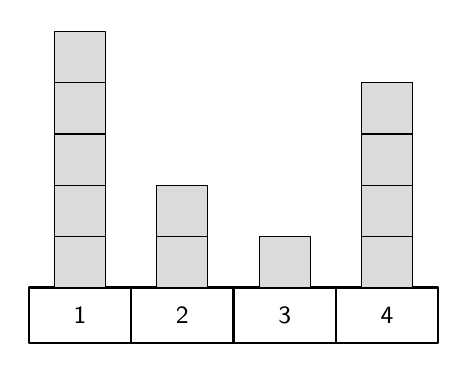
\begin{tikzpicture}[x=1mm,y=1mm,line join=round]
\path (0,0) rectangle (52,40.0);
\draw[thick, fill=white] (0,0) rectangle (13,7);
\node[font=\small] at (6.5,3.5) {1};
\draw[fill=black!14] (3.25,7.0) rectangle (9.75,13.5);
\draw[fill=black!14] (3.25,13.5) rectangle (9.75,20.0);
\draw[fill=black!14] (3.25,20.0) rectangle (9.75,26.5);
\draw[fill=black!14] (3.25,26.5) rectangle (9.75,33.0);
\draw[fill=black!14] (3.25,33.0) rectangle (9.75,39.5);
\draw[thick, fill=white] (13,0) rectangle (26,7);
\node[font=\small] at (19.5,3.5) {2};
\draw[fill=black!14] (16.25,7.0) rectangle (22.75,13.5);
\draw[fill=black!14] (16.25,13.5) rectangle (22.75,20.0);
\draw[thick, fill=white] (26,0) rectangle (39,7);
\node[font=\small] at (32.5,3.5) {3};
\draw[fill=black!14] (29.25,7.0) rectangle (35.75,13.5);
\draw[thick, fill=white] (39,0) rectangle (52,7);
\node[font=\small] at (45.5,3.5) {4};
\draw[fill=black!14] (42.25,7.0) rectangle (48.75,13.5);
\draw[fill=black!14] (42.25,13.5) rectangle (48.75,20.0);
\draw[fill=black!14] (42.25,20.0) rectangle (48.75,26.5);
\draw[fill=black!14] (42.25,26.5) rectangle (48.75,33.0);
\end{tikzpicture}\hspace{12mm}\raisebox{9mm}{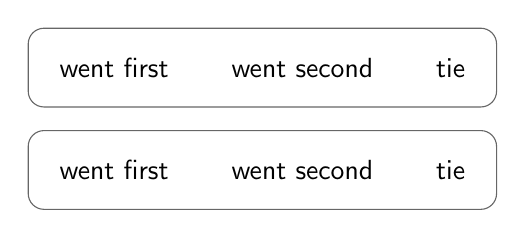
\begin{tikzpicture}[x=1mm,y=1mm]
\node[draw=black!60, rounded corners=2mm, inner xsep=4mm, minimum height=10mm, anchor=west, font=\normalsize] at (0,0) {went first\hspace{8mm}went second\hspace{8mm}tie};
\node[draw=black!60, rounded corners=2mm, inner xsep=4mm, minimum height=10mm, anchor=west, font=\normalsize] at (0,-13) {went first\hspace{8mm}went second\hspace{8mm}tie};
\end{tikzpicture}}\par\vspace{9mm}\noindent\hspace*{4mm}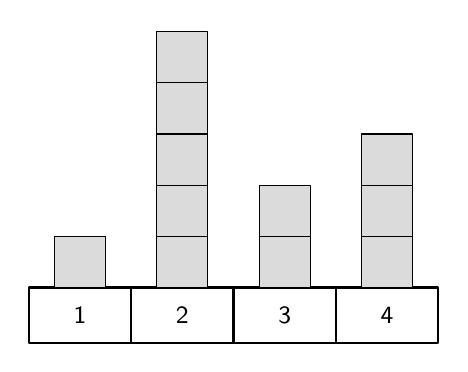
\begin{tikzpicture}[x=1mm,y=1mm,line join=round]
\path (0,0) rectangle (52,40.0);
\draw[thick, fill=white] (0,0) rectangle (13,7);
\node[font=\small] at (6.5,3.5) {1};
\draw[fill=black!14] (3.25,7.0) rectangle (9.75,13.5);
\draw[thick, fill=white] (13,0) rectangle (26,7);
\node[font=\small] at (19.5,3.5) {2};
\draw[fill=black!14] (16.25,7.0) rectangle (22.75,13.5);
\draw[fill=black!14] (16.25,13.5) rectangle (22.75,20.0);
\draw[fill=black!14] (16.25,20.0) rectangle (22.75,26.5);
\draw[fill=black!14] (16.25,26.5) rectangle (22.75,33.0);
\draw[fill=black!14] (16.25,33.0) rectangle (22.75,39.5);
\draw[thick, fill=white] (26,0) rectangle (39,7);
\node[font=\small] at (32.5,3.5) {3};
\draw[fill=black!14] (29.25,7.0) rectangle (35.75,13.5);
\draw[fill=black!14] (29.25,13.5) rectangle (35.75,20.0);
\draw[thick, fill=white] (39,0) rectangle (52,7);
\node[font=\small] at (45.5,3.5) {4};
\draw[fill=black!14] (42.25,7.0) rectangle (48.75,13.5);
\draw[fill=black!14] (42.25,13.5) rectangle (48.75,20.0);
\draw[fill=black!14] (42.25,20.0) rectangle (48.75,26.5);
\end{tikzpicture}\hspace{12mm}\raisebox{9mm}{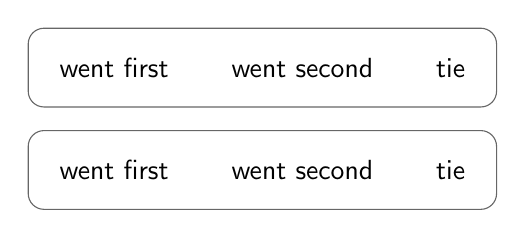
\begin{tikzpicture}[x=1mm,y=1mm]
\node[draw=black!60, rounded corners=2mm, inner xsep=4mm, minimum height=10mm, anchor=west, font=\normalsize] at (0,0) {went first\hspace{8mm}went second\hspace{8mm}tie};
\node[draw=black!60, rounded corners=2mm, inner xsep=4mm, minimum height=10mm, anchor=west, font=\normalsize] at (0,-13) {went first\hspace{8mm}went second\hspace{8mm}tie};
\end{tikzpicture}}\par\vspace{9mm}\noindent\hspace*{4mm}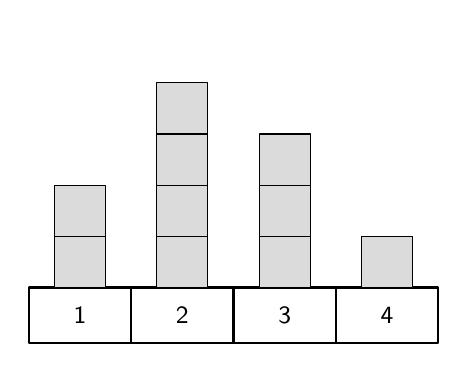
\begin{tikzpicture}[x=1mm,y=1mm,line join=round]
\path (0,0) rectangle (52,40.0);
\draw[thick, fill=white] (0,0) rectangle (13,7);
\node[font=\small] at (6.5,3.5) {1};
\draw[fill=black!14] (3.25,7.0) rectangle (9.75,13.5);
\draw[fill=black!14] (3.25,13.5) rectangle (9.75,20.0);
\draw[thick, fill=white] (13,0) rectangle (26,7);
\node[font=\small] at (19.5,3.5) {2};
\draw[fill=black!14] (16.25,7.0) rectangle (22.75,13.5);
\draw[fill=black!14] (16.25,13.5) rectangle (22.75,20.0);
\draw[fill=black!14] (16.25,20.0) rectangle (22.75,26.5);
\draw[fill=black!14] (16.25,26.5) rectangle (22.75,33.0);
\draw[thick, fill=white] (26,0) rectangle (39,7);
\node[font=\small] at (32.5,3.5) {3};
\draw[fill=black!14] (29.25,7.0) rectangle (35.75,13.5);
\draw[fill=black!14] (29.25,13.5) rectangle (35.75,20.0);
\draw[fill=black!14] (29.25,20.0) rectangle (35.75,26.5);
\draw[thick, fill=white] (39,0) rectangle (52,7);
\node[font=\small] at (45.5,3.5) {4};
\draw[fill=black!14] (42.25,7.0) rectangle (48.75,13.5);
\end{tikzpicture}\hspace{12mm}\raisebox{9mm}{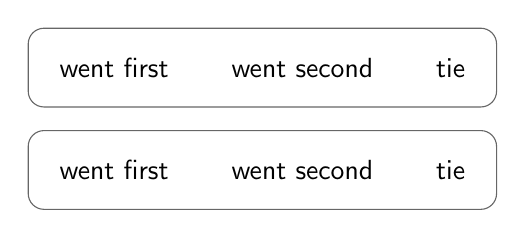
\begin{tikzpicture}[x=1mm,y=1mm]
\node[draw=black!60, rounded corners=2mm, inner xsep=4mm, minimum height=10mm, anchor=west, font=\normalsize] at (0,0) {went first\hspace{8mm}went second\hspace{8mm}tie};
\node[draw=black!60, rounded corners=2mm, inner xsep=4mm, minimum height=10mm, anchor=west, font=\normalsize] at (0,-13) {went first\hspace{8mm}went second\hspace{8mm}tie};
\end{tikzpicture}}\par\vspace{9mm}\newpage\problem You go first. Which tower should you take first so that you win, however your partner plays? Ring it.\par\vspace{8mm}\noindent \begin{minipage}[b]{0.48\linewidth}\centering 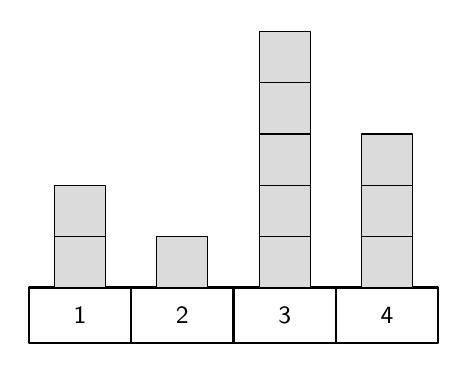
\begin{tikzpicture}[x=1mm,y=1mm,line join=round]
\path (0,0) rectangle (52,40.0);
\draw[thick, fill=white] (0,0) rectangle (13,7);
\node[font=\small] at (6.5,3.5) {1};
\draw[fill=black!14] (3.25,7.0) rectangle (9.75,13.5);
\draw[fill=black!14] (3.25,13.5) rectangle (9.75,20.0);
\draw[thick, fill=white] (13,0) rectangle (26,7);
\node[font=\small] at (19.5,3.5) {2};
\draw[fill=black!14] (16.25,7.0) rectangle (22.75,13.5);
\draw[thick, fill=white] (26,0) rectangle (39,7);
\node[font=\small] at (32.5,3.5) {3};
\draw[fill=black!14] (29.25,7.0) rectangle (35.75,13.5);
\draw[fill=black!14] (29.25,13.5) rectangle (35.75,20.0);
\draw[fill=black!14] (29.25,20.0) rectangle (35.75,26.5);
\draw[fill=black!14] (29.25,26.5) rectangle (35.75,33.0);
\draw[fill=black!14] (29.25,33.0) rectangle (35.75,39.5);
\draw[thick, fill=white] (39,0) rectangle (52,7);
\node[font=\small] at (45.5,3.5) {4};
\draw[fill=black!14] (42.25,7.0) rectangle (48.75,13.5);
\draw[fill=black!14] (42.25,13.5) rectangle (48.75,20.0);
\draw[fill=black!14] (42.25,20.0) rectangle (48.75,26.5);
\end{tikzpicture}\end{minipage}\hfill\begin{minipage}[b]{0.48\linewidth}\centering 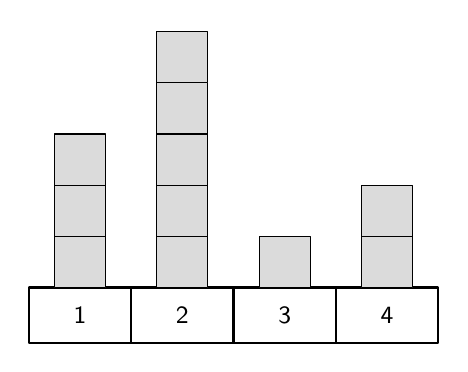
\begin{tikzpicture}[x=1mm,y=1mm,line join=round]
\path (0,0) rectangle (52,40.0);
\draw[thick, fill=white] (0,0) rectangle (13,7);
\node[font=\small] at (6.5,3.5) {1};
\draw[fill=black!14] (3.25,7.0) rectangle (9.75,13.5);
\draw[fill=black!14] (3.25,13.5) rectangle (9.75,20.0);
\draw[fill=black!14] (3.25,20.0) rectangle (9.75,26.5);
\draw[thick, fill=white] (13,0) rectangle (26,7);
\node[font=\small] at (19.5,3.5) {2};
\draw[fill=black!14] (16.25,7.0) rectangle (22.75,13.5);
\draw[fill=black!14] (16.25,13.5) rectangle (22.75,20.0);
\draw[fill=black!14] (16.25,20.0) rectangle (22.75,26.5);
\draw[fill=black!14] (16.25,26.5) rectangle (22.75,33.0);
\draw[fill=black!14] (16.25,33.0) rectangle (22.75,39.5);
\draw[thick, fill=white] (26,0) rectangle (39,7);
\node[font=\small] at (32.5,3.5) {3};
\draw[fill=black!14] (29.25,7.0) rectangle (35.75,13.5);
\draw[thick, fill=white] (39,0) rectangle (52,7);
\node[font=\small] at (45.5,3.5) {4};
\draw[fill=black!14] (42.25,7.0) rectangle (48.75,13.5);
\draw[fill=black!14] (42.25,13.5) rectangle (48.75,20.0);
\end{tikzpicture}\end{minipage}\par\vspace{12mm}
\noindent \begin{minipage}[b]{0.48\linewidth}\centering 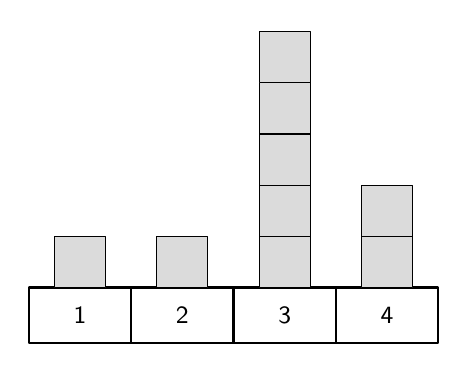
\begin{tikzpicture}[x=1mm,y=1mm,line join=round]
\path (0,0) rectangle (52,40.0);
\draw[thick, fill=white] (0,0) rectangle (13,7);
\node[font=\small] at (6.5,3.5) {1};
\draw[fill=black!14] (3.25,7.0) rectangle (9.75,13.5);
\draw[thick, fill=white] (13,0) rectangle (26,7);
\node[font=\small] at (19.5,3.5) {2};
\draw[fill=black!14] (16.25,7.0) rectangle (22.75,13.5);
\draw[thick, fill=white] (26,0) rectangle (39,7);
\node[font=\small] at (32.5,3.5) {3};
\draw[fill=black!14] (29.25,7.0) rectangle (35.75,13.5);
\draw[fill=black!14] (29.25,13.5) rectangle (35.75,20.0);
\draw[fill=black!14] (29.25,20.0) rectangle (35.75,26.5);
\draw[fill=black!14] (29.25,26.5) rectangle (35.75,33.0);
\draw[fill=black!14] (29.25,33.0) rectangle (35.75,39.5);
\draw[thick, fill=white] (39,0) rectangle (52,7);
\node[font=\small] at (45.5,3.5) {4};
\draw[fill=black!14] (42.25,7.0) rectangle (48.75,13.5);
\draw[fill=black!14] (42.25,13.5) rectangle (48.75,20.0);
\end{tikzpicture}\end{minipage}\hfill\begin{minipage}[b]{0.48\linewidth}\centering 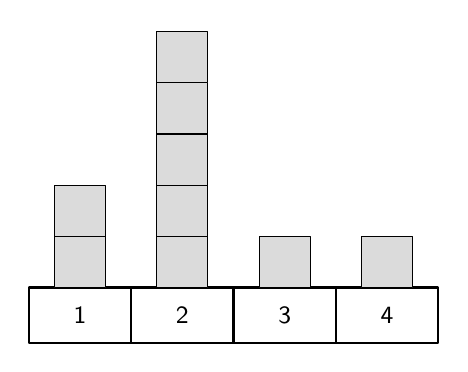
\begin{tikzpicture}[x=1mm,y=1mm,line join=round]
\path (0,0) rectangle (52,40.0);
\draw[thick, fill=white] (0,0) rectangle (13,7);
\node[font=\small] at (6.5,3.5) {1};
\draw[fill=black!14] (3.25,7.0) rectangle (9.75,13.5);
\draw[fill=black!14] (3.25,13.5) rectangle (9.75,20.0);
\draw[thick, fill=white] (13,0) rectangle (26,7);
\node[font=\small] at (19.5,3.5) {2};
\draw[fill=black!14] (16.25,7.0) rectangle (22.75,13.5);
\draw[fill=black!14] (16.25,13.5) rectangle (22.75,20.0);
\draw[fill=black!14] (16.25,20.0) rectangle (22.75,26.5);
\draw[fill=black!14] (16.25,26.5) rectangle (22.75,33.0);
\draw[fill=black!14] (16.25,33.0) rectangle (22.75,39.5);
\draw[thick, fill=white] (26,0) rectangle (39,7);
\node[font=\small] at (32.5,3.5) {3};
\draw[fill=black!14] (29.25,7.0) rectangle (35.75,13.5);
\draw[thick, fill=white] (39,0) rectangle (52,7);
\node[font=\small] at (45.5,3.5) {4};
\draw[fill=black!14] (42.25,7.0) rectangle (48.75,13.5);
\end{tikzpicture}\end{minipage}\par\vspace{12mm}
\noindent \begin{minipage}[b]{0.48\linewidth}\centering 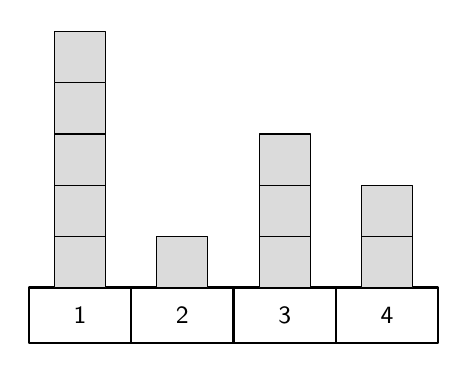
\begin{tikzpicture}[x=1mm,y=1mm,line join=round]
\path (0,0) rectangle (52,40.0);
\draw[thick, fill=white] (0,0) rectangle (13,7);
\node[font=\small] at (6.5,3.5) {1};
\draw[fill=black!14] (3.25,7.0) rectangle (9.75,13.5);
\draw[fill=black!14] (3.25,13.5) rectangle (9.75,20.0);
\draw[fill=black!14] (3.25,20.0) rectangle (9.75,26.5);
\draw[fill=black!14] (3.25,26.5) rectangle (9.75,33.0);
\draw[fill=black!14] (3.25,33.0) rectangle (9.75,39.5);
\draw[thick, fill=white] (13,0) rectangle (26,7);
\node[font=\small] at (19.5,3.5) {2};
\draw[fill=black!14] (16.25,7.0) rectangle (22.75,13.5);
\draw[thick, fill=white] (26,0) rectangle (39,7);
\node[font=\small] at (32.5,3.5) {3};
\draw[fill=black!14] (29.25,7.0) rectangle (35.75,13.5);
\draw[fill=black!14] (29.25,13.5) rectangle (35.75,20.0);
\draw[fill=black!14] (29.25,20.0) rectangle (35.75,26.5);
\draw[thick, fill=white] (39,0) rectangle (52,7);
\node[font=\small] at (45.5,3.5) {4};
\draw[fill=black!14] (42.25,7.0) rectangle (48.75,13.5);
\draw[fill=black!14] (42.25,13.5) rectangle (48.75,20.0);
\end{tikzpicture}\end{minipage}\hfill\begin{minipage}[b]{0.48\linewidth}\centering 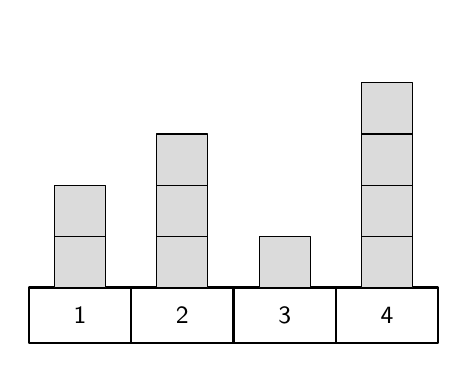
\begin{tikzpicture}[x=1mm,y=1mm,line join=round]
\path (0,0) rectangle (52,40.0);
\draw[thick, fill=white] (0,0) rectangle (13,7);
\node[font=\small] at (6.5,3.5) {1};
\draw[fill=black!14] (3.25,7.0) rectangle (9.75,13.5);
\draw[fill=black!14] (3.25,13.5) rectangle (9.75,20.0);
\draw[thick, fill=white] (13,0) rectangle (26,7);
\node[font=\small] at (19.5,3.5) {2};
\draw[fill=black!14] (16.25,7.0) rectangle (22.75,13.5);
\draw[fill=black!14] (16.25,13.5) rectangle (22.75,20.0);
\draw[fill=black!14] (16.25,20.0) rectangle (22.75,26.5);
\draw[thick, fill=white] (26,0) rectangle (39,7);
\node[font=\small] at (32.5,3.5) {3};
\draw[fill=black!14] (29.25,7.0) rectangle (35.75,13.5);
\draw[thick, fill=white] (39,0) rectangle (52,7);
\node[font=\small] at (45.5,3.5) {4};
\draw[fill=black!14] (42.25,7.0) rectangle (48.75,13.5);
\draw[fill=black!14] (42.25,13.5) rectangle (48.75,20.0);
\draw[fill=black!14] (42.25,20.0) rectangle (48.75,26.5);
\draw[fill=black!14] (42.25,26.5) rectangle (48.75,33.0);
\end{tikzpicture}\end{minipage}\par\vspace{12mm}\newpage\problem Is it better to go first or second on each row? Ring 1st or 2nd.\par\vspace{6mm}\noindent \begin{minipage}[b]{0.48\linewidth}\centering 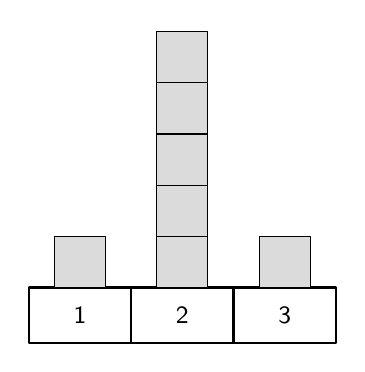
\begin{tikzpicture}[x=1mm,y=1mm,line join=round]
\path (0,0) rectangle (39,40.0);
\draw[thick, fill=white] (0,0) rectangle (13,7);
\node[font=\small] at (6.5,3.5) {1};
\draw[fill=black!14] (3.25,7.0) rectangle (9.75,13.5);
\draw[thick, fill=white] (13,0) rectangle (26,7);
\node[font=\small] at (19.5,3.5) {2};
\draw[fill=black!14] (16.25,7.0) rectangle (22.75,13.5);
\draw[fill=black!14] (16.25,13.5) rectangle (22.75,20.0);
\draw[fill=black!14] (16.25,20.0) rectangle (22.75,26.5);
\draw[fill=black!14] (16.25,26.5) rectangle (22.75,33.0);
\draw[fill=black!14] (16.25,33.0) rectangle (22.75,39.5);
\draw[thick, fill=white] (26,0) rectangle (39,7);
\node[font=\small] at (32.5,3.5) {3};
\draw[fill=black!14] (29.25,7.0) rectangle (35.75,13.5);
\end{tikzpicture}\\[3mm]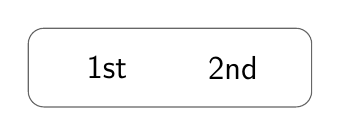
\begin{tikzpicture}[x=1mm,y=1mm]
\draw[rounded corners=2mm, black!60] (0,0) rectangle (36,10);
\node[font=\large] at (10,5) {1st};
\node[font=\large] at (26,5) {2nd};
\end{tikzpicture}\end{minipage}\hfill\begin{minipage}[b]{0.48\linewidth}\centering 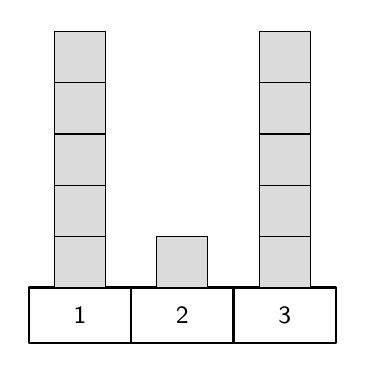
\begin{tikzpicture}[x=1mm,y=1mm,line join=round]
\path (0,0) rectangle (39,40.0);
\draw[thick, fill=white] (0,0) rectangle (13,7);
\node[font=\small] at (6.5,3.5) {1};
\draw[fill=black!14] (3.25,7.0) rectangle (9.75,13.5);
\draw[fill=black!14] (3.25,13.5) rectangle (9.75,20.0);
\draw[fill=black!14] (3.25,20.0) rectangle (9.75,26.5);
\draw[fill=black!14] (3.25,26.5) rectangle (9.75,33.0);
\draw[fill=black!14] (3.25,33.0) rectangle (9.75,39.5);
\draw[thick, fill=white] (13,0) rectangle (26,7);
\node[font=\small] at (19.5,3.5) {2};
\draw[fill=black!14] (16.25,7.0) rectangle (22.75,13.5);
\draw[thick, fill=white] (26,0) rectangle (39,7);
\node[font=\small] at (32.5,3.5) {3};
\draw[fill=black!14] (29.25,7.0) rectangle (35.75,13.5);
\draw[fill=black!14] (29.25,13.5) rectangle (35.75,20.0);
\draw[fill=black!14] (29.25,20.0) rectangle (35.75,26.5);
\draw[fill=black!14] (29.25,26.5) rectangle (35.75,33.0);
\draw[fill=black!14] (29.25,33.0) rectangle (35.75,39.5);
\end{tikzpicture}\\[3mm]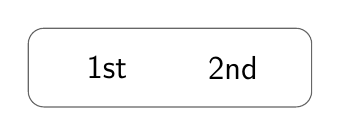
\begin{tikzpicture}[x=1mm,y=1mm]
\draw[rounded corners=2mm, black!60] (0,0) rectangle (36,10);
\node[font=\large] at (10,5) {1st};
\node[font=\large] at (26,5) {2nd};
\end{tikzpicture}\end{minipage}\par\vspace{9mm}
\noindent \begin{minipage}[b]{0.48\linewidth}\centering 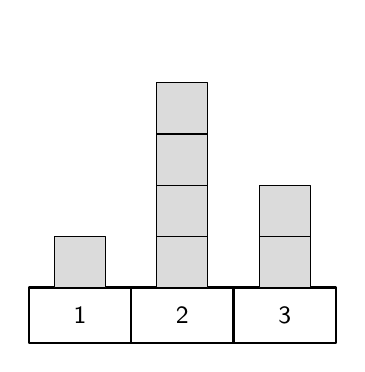
\begin{tikzpicture}[x=1mm,y=1mm,line join=round]
\path (0,0) rectangle (39,40.0);
\draw[thick, fill=white] (0,0) rectangle (13,7);
\node[font=\small] at (6.5,3.5) {1};
\draw[fill=black!14] (3.25,7.0) rectangle (9.75,13.5);
\draw[thick, fill=white] (13,0) rectangle (26,7);
\node[font=\small] at (19.5,3.5) {2};
\draw[fill=black!14] (16.25,7.0) rectangle (22.75,13.5);
\draw[fill=black!14] (16.25,13.5) rectangle (22.75,20.0);
\draw[fill=black!14] (16.25,20.0) rectangle (22.75,26.5);
\draw[fill=black!14] (16.25,26.5) rectangle (22.75,33.0);
\draw[thick, fill=white] (26,0) rectangle (39,7);
\node[font=\small] at (32.5,3.5) {3};
\draw[fill=black!14] (29.25,7.0) rectangle (35.75,13.5);
\draw[fill=black!14] (29.25,13.5) rectangle (35.75,20.0);
\end{tikzpicture}\\[3mm]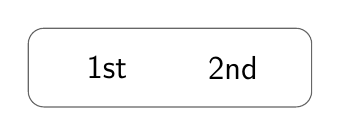
\begin{tikzpicture}[x=1mm,y=1mm]
\draw[rounded corners=2mm, black!60] (0,0) rectangle (36,10);
\node[font=\large] at (10,5) {1st};
\node[font=\large] at (26,5) {2nd};
\end{tikzpicture}\end{minipage}\hfill\begin{minipage}[b]{0.48\linewidth}\centering 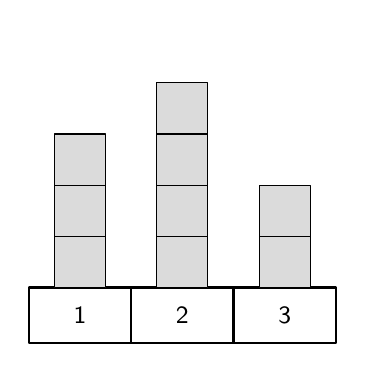
\begin{tikzpicture}[x=1mm,y=1mm,line join=round]
\path (0,0) rectangle (39,40.0);
\draw[thick, fill=white] (0,0) rectangle (13,7);
\node[font=\small] at (6.5,3.5) {1};
\draw[fill=black!14] (3.25,7.0) rectangle (9.75,13.5);
\draw[fill=black!14] (3.25,13.5) rectangle (9.75,20.0);
\draw[fill=black!14] (3.25,20.0) rectangle (9.75,26.5);
\draw[thick, fill=white] (13,0) rectangle (26,7);
\node[font=\small] at (19.5,3.5) {2};
\draw[fill=black!14] (16.25,7.0) rectangle (22.75,13.5);
\draw[fill=black!14] (16.25,13.5) rectangle (22.75,20.0);
\draw[fill=black!14] (16.25,20.0) rectangle (22.75,26.5);
\draw[fill=black!14] (16.25,26.5) rectangle (22.75,33.0);
\draw[thick, fill=white] (26,0) rectangle (39,7);
\node[font=\small] at (32.5,3.5) {3};
\draw[fill=black!14] (29.25,7.0) rectangle (35.75,13.5);
\draw[fill=black!14] (29.25,13.5) rectangle (35.75,20.0);
\end{tikzpicture}\\[3mm]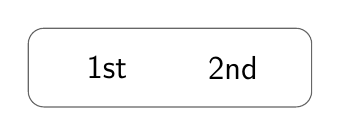
\begin{tikzpicture}[x=1mm,y=1mm]
\draw[rounded corners=2mm, black!60] (0,0) rectangle (36,10);
\node[font=\large] at (10,5) {1st};
\node[font=\large] at (26,5) {2nd};
\end{tikzpicture}\end{minipage}\par\vspace{9mm}
\noindent \begin{minipage}[b]{0.48\linewidth}\centering 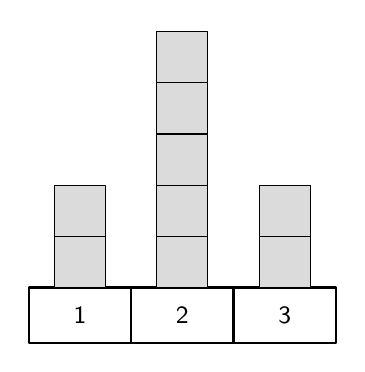
\begin{tikzpicture}[x=1mm,y=1mm,line join=round]
\path (0,0) rectangle (39,40.0);
\draw[thick, fill=white] (0,0) rectangle (13,7);
\node[font=\small] at (6.5,3.5) {1};
\draw[fill=black!14] (3.25,7.0) rectangle (9.75,13.5);
\draw[fill=black!14] (3.25,13.5) rectangle (9.75,20.0);
\draw[thick, fill=white] (13,0) rectangle (26,7);
\node[font=\small] at (19.5,3.5) {2};
\draw[fill=black!14] (16.25,7.0) rectangle (22.75,13.5);
\draw[fill=black!14] (16.25,13.5) rectangle (22.75,20.0);
\draw[fill=black!14] (16.25,20.0) rectangle (22.75,26.5);
\draw[fill=black!14] (16.25,26.5) rectangle (22.75,33.0);
\draw[fill=black!14] (16.25,33.0) rectangle (22.75,39.5);
\draw[thick, fill=white] (26,0) rectangle (39,7);
\node[font=\small] at (32.5,3.5) {3};
\draw[fill=black!14] (29.25,7.0) rectangle (35.75,13.5);
\draw[fill=black!14] (29.25,13.5) rectangle (35.75,20.0);
\end{tikzpicture}\\[3mm]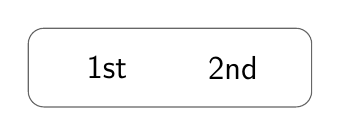
\begin{tikzpicture}[x=1mm,y=1mm]
\draw[rounded corners=2mm, black!60] (0,0) rectangle (36,10);
\node[font=\large] at (10,5) {1st};
\node[font=\large] at (26,5) {2nd};
\end{tikzpicture}\end{minipage}\hfill\null\par\vspace{9mm}\newpage\problem Make up rows of three towers where whoever goes first loses. Draw them.\par\vspace{7mm}\noindent \begin{minipage}[b]{0.48\linewidth}\centering 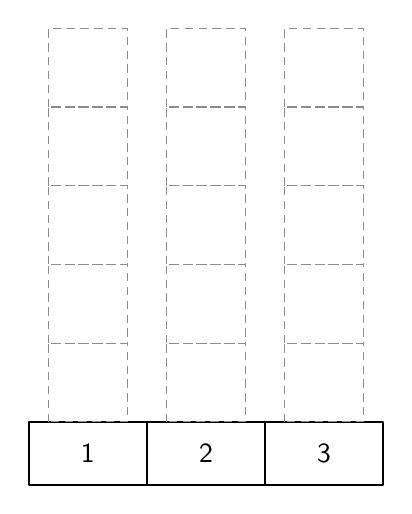
\begin{tikzpicture}[x=1mm,y=1mm,line join=round]
\draw[thick, fill=white] (0,0) rectangle (15,8);
\node[font=\normalsize] at (7.5,4.0) {1};
\draw[black!45, densely dashed] (2.5,8) rectangle (12.5,18);
\draw[black!45, densely dashed] (2.5,18) rectangle (12.5,28);
\draw[black!45, densely dashed] (2.5,28) rectangle (12.5,38);
\draw[black!45, densely dashed] (2.5,38) rectangle (12.5,48);
\draw[black!45, densely dashed] (2.5,48) rectangle (12.5,58);
\draw[thick, fill=white] (15,0) rectangle (30,8);
\node[font=\normalsize] at (22.5,4.0) {2};
\draw[black!45, densely dashed] (17.5,8) rectangle (27.5,18);
\draw[black!45, densely dashed] (17.5,18) rectangle (27.5,28);
\draw[black!45, densely dashed] (17.5,28) rectangle (27.5,38);
\draw[black!45, densely dashed] (17.5,38) rectangle (27.5,48);
\draw[black!45, densely dashed] (17.5,48) rectangle (27.5,58);
\draw[thick, fill=white] (30,0) rectangle (45,8);
\node[font=\normalsize] at (37.5,4.0) {3};
\draw[black!45, densely dashed] (32.5,8) rectangle (42.5,18);
\draw[black!45, densely dashed] (32.5,18) rectangle (42.5,28);
\draw[black!45, densely dashed] (32.5,28) rectangle (42.5,38);
\draw[black!45, densely dashed] (32.5,38) rectangle (42.5,48);
\draw[black!45, densely dashed] (32.5,48) rectangle (42.5,58);
\end{tikzpicture}\end{minipage}\hfill\begin{minipage}[b]{0.48\linewidth}\centering 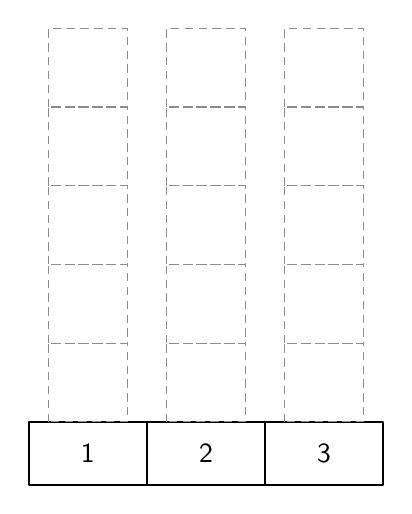
\begin{tikzpicture}[x=1mm,y=1mm,line join=round]
\draw[thick, fill=white] (0,0) rectangle (15,8);
\node[font=\normalsize] at (7.5,4.0) {1};
\draw[black!45, densely dashed] (2.5,8) rectangle (12.5,18);
\draw[black!45, densely dashed] (2.5,18) rectangle (12.5,28);
\draw[black!45, densely dashed] (2.5,28) rectangle (12.5,38);
\draw[black!45, densely dashed] (2.5,38) rectangle (12.5,48);
\draw[black!45, densely dashed] (2.5,48) rectangle (12.5,58);
\draw[thick, fill=white] (15,0) rectangle (30,8);
\node[font=\normalsize] at (22.5,4.0) {2};
\draw[black!45, densely dashed] (17.5,8) rectangle (27.5,18);
\draw[black!45, densely dashed] (17.5,18) rectangle (27.5,28);
\draw[black!45, densely dashed] (17.5,28) rectangle (27.5,38);
\draw[black!45, densely dashed] (17.5,38) rectangle (27.5,48);
\draw[black!45, densely dashed] (17.5,48) rectangle (27.5,58);
\draw[thick, fill=white] (30,0) rectangle (45,8);
\node[font=\normalsize] at (37.5,4.0) {3};
\draw[black!45, densely dashed] (32.5,8) rectangle (42.5,18);
\draw[black!45, densely dashed] (32.5,18) rectangle (42.5,28);
\draw[black!45, densely dashed] (32.5,28) rectangle (42.5,38);
\draw[black!45, densely dashed] (32.5,38) rectangle (42.5,48);
\draw[black!45, densely dashed] (32.5,48) rectangle (42.5,58);
\end{tikzpicture}\end{minipage}\par\vspace{11mm}
\noindent \begin{minipage}[b]{0.48\linewidth}\centering 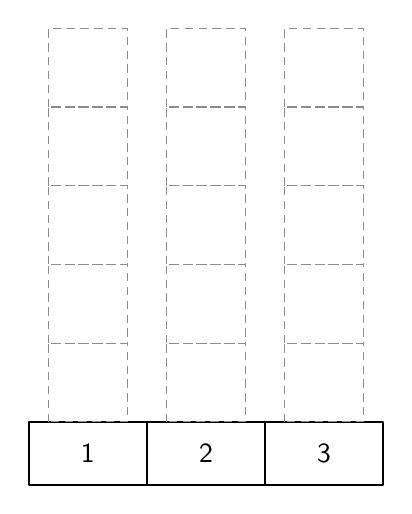
\begin{tikzpicture}[x=1mm,y=1mm,line join=round]
\draw[thick, fill=white] (0,0) rectangle (15,8);
\node[font=\normalsize] at (7.5,4.0) {1};
\draw[black!45, densely dashed] (2.5,8) rectangle (12.5,18);
\draw[black!45, densely dashed] (2.5,18) rectangle (12.5,28);
\draw[black!45, densely dashed] (2.5,28) rectangle (12.5,38);
\draw[black!45, densely dashed] (2.5,38) rectangle (12.5,48);
\draw[black!45, densely dashed] (2.5,48) rectangle (12.5,58);
\draw[thick, fill=white] (15,0) rectangle (30,8);
\node[font=\normalsize] at (22.5,4.0) {2};
\draw[black!45, densely dashed] (17.5,8) rectangle (27.5,18);
\draw[black!45, densely dashed] (17.5,18) rectangle (27.5,28);
\draw[black!45, densely dashed] (17.5,28) rectangle (27.5,38);
\draw[black!45, densely dashed] (17.5,38) rectangle (27.5,48);
\draw[black!45, densely dashed] (17.5,48) rectangle (27.5,58);
\draw[thick, fill=white] (30,0) rectangle (45,8);
\node[font=\normalsize] at (37.5,4.0) {3};
\draw[black!45, densely dashed] (32.5,8) rectangle (42.5,18);
\draw[black!45, densely dashed] (32.5,18) rectangle (42.5,28);
\draw[black!45, densely dashed] (32.5,28) rectangle (42.5,38);
\draw[black!45, densely dashed] (32.5,38) rectangle (42.5,48);
\draw[black!45, densely dashed] (32.5,48) rectangle (42.5,58);
\end{tikzpicture}\end{minipage}\hfill\begin{minipage}[b]{0.48\linewidth}\centering 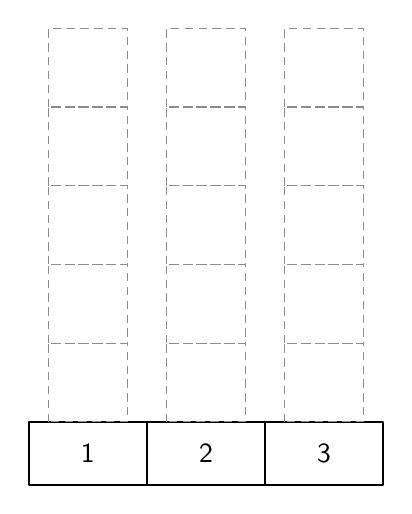
\begin{tikzpicture}[x=1mm,y=1mm,line join=round]
\draw[thick, fill=white] (0,0) rectangle (15,8);
\node[font=\normalsize] at (7.5,4.0) {1};
\draw[black!45, densely dashed] (2.5,8) rectangle (12.5,18);
\draw[black!45, densely dashed] (2.5,18) rectangle (12.5,28);
\draw[black!45, densely dashed] (2.5,28) rectangle (12.5,38);
\draw[black!45, densely dashed] (2.5,38) rectangle (12.5,48);
\draw[black!45, densely dashed] (2.5,48) rectangle (12.5,58);
\draw[thick, fill=white] (15,0) rectangle (30,8);
\node[font=\normalsize] at (22.5,4.0) {2};
\draw[black!45, densely dashed] (17.5,8) rectangle (27.5,18);
\draw[black!45, densely dashed] (17.5,18) rectangle (27.5,28);
\draw[black!45, densely dashed] (17.5,28) rectangle (27.5,38);
\draw[black!45, densely dashed] (17.5,38) rectangle (27.5,48);
\draw[black!45, densely dashed] (17.5,48) rectangle (27.5,58);
\draw[thick, fill=white] (30,0) rectangle (45,8);
\node[font=\normalsize] at (37.5,4.0) {3};
\draw[black!45, densely dashed] (32.5,8) rectangle (42.5,18);
\draw[black!45, densely dashed] (32.5,18) rectangle (42.5,28);
\draw[black!45, densely dashed] (32.5,28) rectangle (42.5,38);
\draw[black!45, densely dashed] (32.5,38) rectangle (42.5,48);
\draw[black!45, densely dashed] (32.5,48) rectangle (42.5,58);
\end{tikzpicture}\end{minipage}\par\vspace{11mm}
\noindent \begin{minipage}[b]{0.48\linewidth}\centering 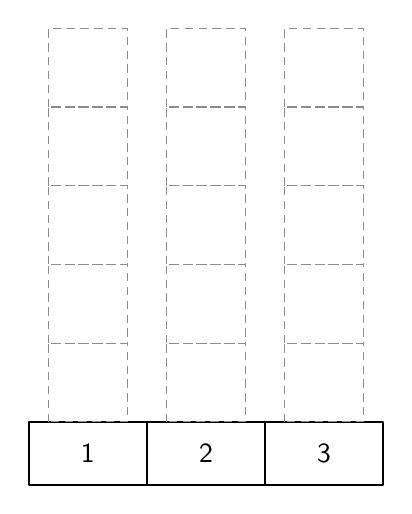
\begin{tikzpicture}[x=1mm,y=1mm,line join=round]
\draw[thick, fill=white] (0,0) rectangle (15,8);
\node[font=\normalsize] at (7.5,4.0) {1};
\draw[black!45, densely dashed] (2.5,8) rectangle (12.5,18);
\draw[black!45, densely dashed] (2.5,18) rectangle (12.5,28);
\draw[black!45, densely dashed] (2.5,28) rectangle (12.5,38);
\draw[black!45, densely dashed] (2.5,38) rectangle (12.5,48);
\draw[black!45, densely dashed] (2.5,48) rectangle (12.5,58);
\draw[thick, fill=white] (15,0) rectangle (30,8);
\node[font=\normalsize] at (22.5,4.0) {2};
\draw[black!45, densely dashed] (17.5,8) rectangle (27.5,18);
\draw[black!45, densely dashed] (17.5,18) rectangle (27.5,28);
\draw[black!45, densely dashed] (17.5,28) rectangle (27.5,38);
\draw[black!45, densely dashed] (17.5,38) rectangle (27.5,48);
\draw[black!45, densely dashed] (17.5,48) rectangle (27.5,58);
\draw[thick, fill=white] (30,0) rectangle (45,8);
\node[font=\normalsize] at (37.5,4.0) {3};
\draw[black!45, densely dashed] (32.5,8) rectangle (42.5,18);
\draw[black!45, densely dashed] (32.5,18) rectangle (42.5,28);
\draw[black!45, densely dashed] (32.5,28) rectangle (42.5,38);
\draw[black!45, densely dashed] (32.5,38) rectangle (42.5,48);
\draw[black!45, densely dashed] (32.5,48) rectangle (42.5,58);
\end{tikzpicture}\end{minipage}\hfill\begin{minipage}[b]{0.48\linewidth}\centering 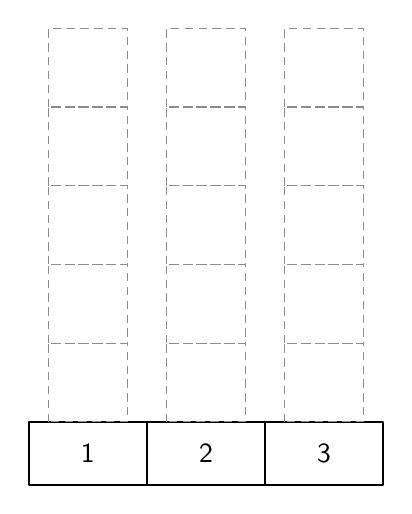
\begin{tikzpicture}[x=1mm,y=1mm,line join=round]
\draw[thick, fill=white] (0,0) rectangle (15,8);
\node[font=\normalsize] at (7.5,4.0) {1};
\draw[black!45, densely dashed] (2.5,8) rectangle (12.5,18);
\draw[black!45, densely dashed] (2.5,18) rectangle (12.5,28);
\draw[black!45, densely dashed] (2.5,28) rectangle (12.5,38);
\draw[black!45, densely dashed] (2.5,38) rectangle (12.5,48);
\draw[black!45, densely dashed] (2.5,48) rectangle (12.5,58);
\draw[thick, fill=white] (15,0) rectangle (30,8);
\node[font=\normalsize] at (22.5,4.0) {2};
\draw[black!45, densely dashed] (17.5,8) rectangle (27.5,18);
\draw[black!45, densely dashed] (17.5,18) rectangle (27.5,28);
\draw[black!45, densely dashed] (17.5,28) rectangle (27.5,38);
\draw[black!45, densely dashed] (17.5,38) rectangle (27.5,48);
\draw[black!45, densely dashed] (17.5,48) rectangle (27.5,58);
\draw[thick, fill=white] (30,0) rectangle (45,8);
\node[font=\normalsize] at (37.5,4.0) {3};
\draw[black!45, densely dashed] (32.5,8) rectangle (42.5,18);
\draw[black!45, densely dashed] (32.5,18) rectangle (42.5,28);
\draw[black!45, densely dashed] (32.5,28) rectangle (42.5,38);
\draw[black!45, densely dashed] (32.5,38) rectangle (42.5,48);
\draw[black!45, densely dashed] (32.5,48) rectangle (42.5,58);
\end{tikzpicture}\end{minipage}\par\vspace{11mm}\newpage\problem Can you make a row of four towers where whoever goes first loses?\par\vspace{7mm}\noindent \begin{minipage}[b]{0.48\linewidth}\centering 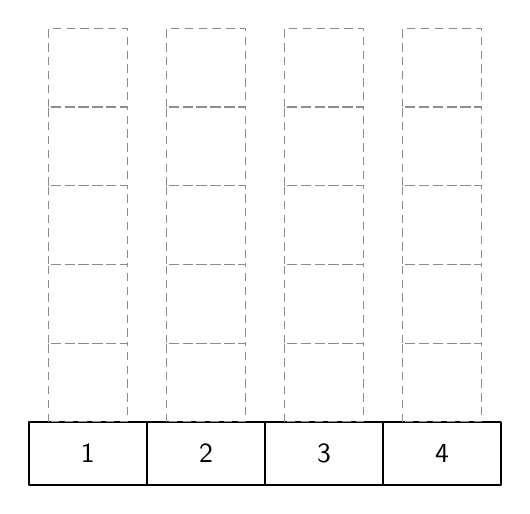
\begin{tikzpicture}[x=1mm,y=1mm,line join=round]
\draw[thick, fill=white] (0,0) rectangle (15,8);
\node[font=\normalsize] at (7.5,4.0) {1};
\draw[black!45, densely dashed] (2.5,8) rectangle (12.5,18);
\draw[black!45, densely dashed] (2.5,18) rectangle (12.5,28);
\draw[black!45, densely dashed] (2.5,28) rectangle (12.5,38);
\draw[black!45, densely dashed] (2.5,38) rectangle (12.5,48);
\draw[black!45, densely dashed] (2.5,48) rectangle (12.5,58);
\draw[thick, fill=white] (15,0) rectangle (30,8);
\node[font=\normalsize] at (22.5,4.0) {2};
\draw[black!45, densely dashed] (17.5,8) rectangle (27.5,18);
\draw[black!45, densely dashed] (17.5,18) rectangle (27.5,28);
\draw[black!45, densely dashed] (17.5,28) rectangle (27.5,38);
\draw[black!45, densely dashed] (17.5,38) rectangle (27.5,48);
\draw[black!45, densely dashed] (17.5,48) rectangle (27.5,58);
\draw[thick, fill=white] (30,0) rectangle (45,8);
\node[font=\normalsize] at (37.5,4.0) {3};
\draw[black!45, densely dashed] (32.5,8) rectangle (42.5,18);
\draw[black!45, densely dashed] (32.5,18) rectangle (42.5,28);
\draw[black!45, densely dashed] (32.5,28) rectangle (42.5,38);
\draw[black!45, densely dashed] (32.5,38) rectangle (42.5,48);
\draw[black!45, densely dashed] (32.5,48) rectangle (42.5,58);
\draw[thick, fill=white] (45,0) rectangle (60,8);
\node[font=\normalsize] at (52.5,4.0) {4};
\draw[black!45, densely dashed] (47.5,8) rectangle (57.5,18);
\draw[black!45, densely dashed] (47.5,18) rectangle (57.5,28);
\draw[black!45, densely dashed] (47.5,28) rectangle (57.5,38);
\draw[black!45, densely dashed] (47.5,38) rectangle (57.5,48);
\draw[black!45, densely dashed] (47.5,48) rectangle (57.5,58);
\end{tikzpicture}\end{minipage}\hfill\begin{minipage}[b]{0.48\linewidth}\centering 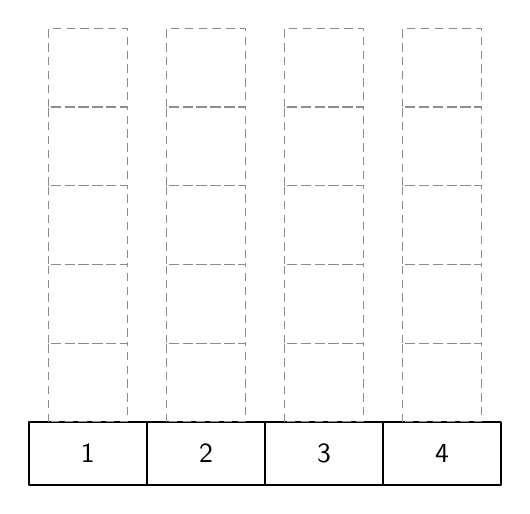
\begin{tikzpicture}[x=1mm,y=1mm,line join=round]
\draw[thick, fill=white] (0,0) rectangle (15,8);
\node[font=\normalsize] at (7.5,4.0) {1};
\draw[black!45, densely dashed] (2.5,8) rectangle (12.5,18);
\draw[black!45, densely dashed] (2.5,18) rectangle (12.5,28);
\draw[black!45, densely dashed] (2.5,28) rectangle (12.5,38);
\draw[black!45, densely dashed] (2.5,38) rectangle (12.5,48);
\draw[black!45, densely dashed] (2.5,48) rectangle (12.5,58);
\draw[thick, fill=white] (15,0) rectangle (30,8);
\node[font=\normalsize] at (22.5,4.0) {2};
\draw[black!45, densely dashed] (17.5,8) rectangle (27.5,18);
\draw[black!45, densely dashed] (17.5,18) rectangle (27.5,28);
\draw[black!45, densely dashed] (17.5,28) rectangle (27.5,38);
\draw[black!45, densely dashed] (17.5,38) rectangle (27.5,48);
\draw[black!45, densely dashed] (17.5,48) rectangle (27.5,58);
\draw[thick, fill=white] (30,0) rectangle (45,8);
\node[font=\normalsize] at (37.5,4.0) {3};
\draw[black!45, densely dashed] (32.5,8) rectangle (42.5,18);
\draw[black!45, densely dashed] (32.5,18) rectangle (42.5,28);
\draw[black!45, densely dashed] (32.5,28) rectangle (42.5,38);
\draw[black!45, densely dashed] (32.5,38) rectangle (42.5,48);
\draw[black!45, densely dashed] (32.5,48) rectangle (42.5,58);
\draw[thick, fill=white] (45,0) rectangle (60,8);
\node[font=\normalsize] at (52.5,4.0) {4};
\draw[black!45, densely dashed] (47.5,8) rectangle (57.5,18);
\draw[black!45, densely dashed] (47.5,18) rectangle (57.5,28);
\draw[black!45, densely dashed] (47.5,28) rectangle (57.5,38);
\draw[black!45, densely dashed] (47.5,38) rectangle (57.5,48);
\draw[black!45, densely dashed] (47.5,48) rectangle (57.5,58);
\end{tikzpicture}\end{minipage}\par\vspace{11mm}
\noindent \begin{minipage}[b]{0.48\linewidth}\centering 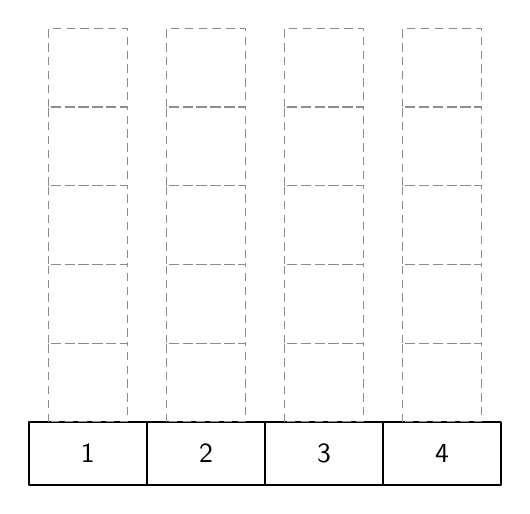
\begin{tikzpicture}[x=1mm,y=1mm,line join=round]
\draw[thick, fill=white] (0,0) rectangle (15,8);
\node[font=\normalsize] at (7.5,4.0) {1};
\draw[black!45, densely dashed] (2.5,8) rectangle (12.5,18);
\draw[black!45, densely dashed] (2.5,18) rectangle (12.5,28);
\draw[black!45, densely dashed] (2.5,28) rectangle (12.5,38);
\draw[black!45, densely dashed] (2.5,38) rectangle (12.5,48);
\draw[black!45, densely dashed] (2.5,48) rectangle (12.5,58);
\draw[thick, fill=white] (15,0) rectangle (30,8);
\node[font=\normalsize] at (22.5,4.0) {2};
\draw[black!45, densely dashed] (17.5,8) rectangle (27.5,18);
\draw[black!45, densely dashed] (17.5,18) rectangle (27.5,28);
\draw[black!45, densely dashed] (17.5,28) rectangle (27.5,38);
\draw[black!45, densely dashed] (17.5,38) rectangle (27.5,48);
\draw[black!45, densely dashed] (17.5,48) rectangle (27.5,58);
\draw[thick, fill=white] (30,0) rectangle (45,8);
\node[font=\normalsize] at (37.5,4.0) {3};
\draw[black!45, densely dashed] (32.5,8) rectangle (42.5,18);
\draw[black!45, densely dashed] (32.5,18) rectangle (42.5,28);
\draw[black!45, densely dashed] (32.5,28) rectangle (42.5,38);
\draw[black!45, densely dashed] (32.5,38) rectangle (42.5,48);
\draw[black!45, densely dashed] (32.5,48) rectangle (42.5,58);
\draw[thick, fill=white] (45,0) rectangle (60,8);
\node[font=\normalsize] at (52.5,4.0) {4};
\draw[black!45, densely dashed] (47.5,8) rectangle (57.5,18);
\draw[black!45, densely dashed] (47.5,18) rectangle (57.5,28);
\draw[black!45, densely dashed] (47.5,28) rectangle (57.5,38);
\draw[black!45, densely dashed] (47.5,38) rectangle (57.5,48);
\draw[black!45, densely dashed] (47.5,48) rectangle (57.5,58);
\end{tikzpicture}\end{minipage}\hfill\begin{minipage}[b]{0.48\linewidth}\centering 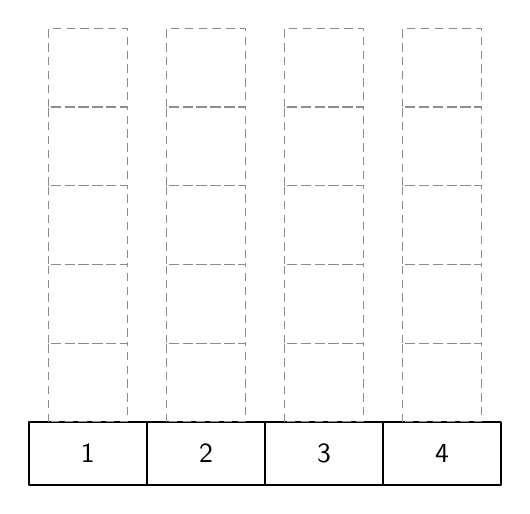
\begin{tikzpicture}[x=1mm,y=1mm,line join=round]
\draw[thick, fill=white] (0,0) rectangle (15,8);
\node[font=\normalsize] at (7.5,4.0) {1};
\draw[black!45, densely dashed] (2.5,8) rectangle (12.5,18);
\draw[black!45, densely dashed] (2.5,18) rectangle (12.5,28);
\draw[black!45, densely dashed] (2.5,28) rectangle (12.5,38);
\draw[black!45, densely dashed] (2.5,38) rectangle (12.5,48);
\draw[black!45, densely dashed] (2.5,48) rectangle (12.5,58);
\draw[thick, fill=white] (15,0) rectangle (30,8);
\node[font=\normalsize] at (22.5,4.0) {2};
\draw[black!45, densely dashed] (17.5,8) rectangle (27.5,18);
\draw[black!45, densely dashed] (17.5,18) rectangle (27.5,28);
\draw[black!45, densely dashed] (17.5,28) rectangle (27.5,38);
\draw[black!45, densely dashed] (17.5,38) rectangle (27.5,48);
\draw[black!45, densely dashed] (17.5,48) rectangle (27.5,58);
\draw[thick, fill=white] (30,0) rectangle (45,8);
\node[font=\normalsize] at (37.5,4.0) {3};
\draw[black!45, densely dashed] (32.5,8) rectangle (42.5,18);
\draw[black!45, densely dashed] (32.5,18) rectangle (42.5,28);
\draw[black!45, densely dashed] (32.5,28) rectangle (42.5,38);
\draw[black!45, densely dashed] (32.5,38) rectangle (42.5,48);
\draw[black!45, densely dashed] (32.5,48) rectangle (42.5,58);
\draw[thick, fill=white] (45,0) rectangle (60,8);
\node[font=\normalsize] at (52.5,4.0) {4};
\draw[black!45, densely dashed] (47.5,8) rectangle (57.5,18);
\draw[black!45, densely dashed] (47.5,18) rectangle (57.5,28);
\draw[black!45, densely dashed] (47.5,28) rectangle (57.5,38);
\draw[black!45, densely dashed] (47.5,38) rectangle (57.5,48);
\draw[black!45, densely dashed] (47.5,48) rectangle (57.5,58);
\end{tikzpicture}\end{minipage}\par\vspace{11mm}
\noindent \begin{minipage}[b]{0.48\linewidth}\centering 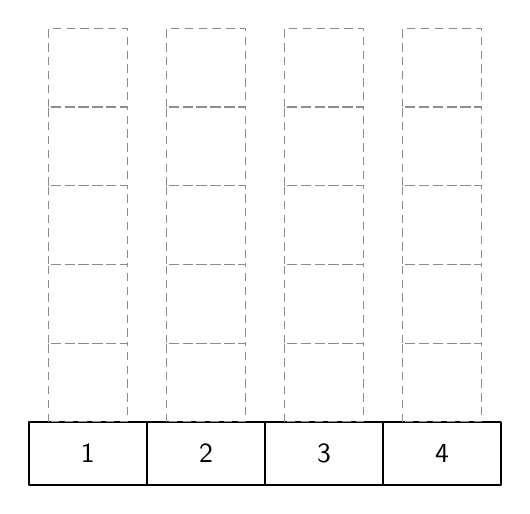
\begin{tikzpicture}[x=1mm,y=1mm,line join=round]
\draw[thick, fill=white] (0,0) rectangle (15,8);
\node[font=\normalsize] at (7.5,4.0) {1};
\draw[black!45, densely dashed] (2.5,8) rectangle (12.5,18);
\draw[black!45, densely dashed] (2.5,18) rectangle (12.5,28);
\draw[black!45, densely dashed] (2.5,28) rectangle (12.5,38);
\draw[black!45, densely dashed] (2.5,38) rectangle (12.5,48);
\draw[black!45, densely dashed] (2.5,48) rectangle (12.5,58);
\draw[thick, fill=white] (15,0) rectangle (30,8);
\node[font=\normalsize] at (22.5,4.0) {2};
\draw[black!45, densely dashed] (17.5,8) rectangle (27.5,18);
\draw[black!45, densely dashed] (17.5,18) rectangle (27.5,28);
\draw[black!45, densely dashed] (17.5,28) rectangle (27.5,38);
\draw[black!45, densely dashed] (17.5,38) rectangle (27.5,48);
\draw[black!45, densely dashed] (17.5,48) rectangle (27.5,58);
\draw[thick, fill=white] (30,0) rectangle (45,8);
\node[font=\normalsize] at (37.5,4.0) {3};
\draw[black!45, densely dashed] (32.5,8) rectangle (42.5,18);
\draw[black!45, densely dashed] (32.5,18) rectangle (42.5,28);
\draw[black!45, densely dashed] (32.5,28) rectangle (42.5,38);
\draw[black!45, densely dashed] (32.5,38) rectangle (42.5,48);
\draw[black!45, densely dashed] (32.5,48) rectangle (42.5,58);
\draw[thick, fill=white] (45,0) rectangle (60,8);
\node[font=\normalsize] at (52.5,4.0) {4};
\draw[black!45, densely dashed] (47.5,8) rectangle (57.5,18);
\draw[black!45, densely dashed] (47.5,18) rectangle (57.5,28);
\draw[black!45, densely dashed] (47.5,28) rectangle (57.5,38);
\draw[black!45, densely dashed] (47.5,38) rectangle (57.5,48);
\draw[black!45, densely dashed] (47.5,48) rectangle (57.5,58);
\end{tikzpicture}\end{minipage}\hfill\begin{minipage}[b]{0.48\linewidth}\centering 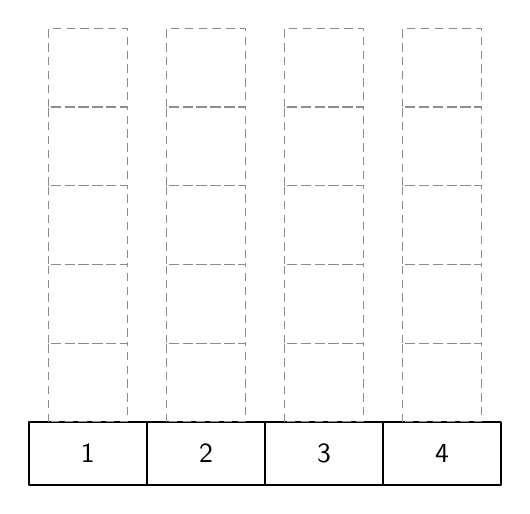
\begin{tikzpicture}[x=1mm,y=1mm,line join=round]
\draw[thick, fill=white] (0,0) rectangle (15,8);
\node[font=\normalsize] at (7.5,4.0) {1};
\draw[black!45, densely dashed] (2.5,8) rectangle (12.5,18);
\draw[black!45, densely dashed] (2.5,18) rectangle (12.5,28);
\draw[black!45, densely dashed] (2.5,28) rectangle (12.5,38);
\draw[black!45, densely dashed] (2.5,38) rectangle (12.5,48);
\draw[black!45, densely dashed] (2.5,48) rectangle (12.5,58);
\draw[thick, fill=white] (15,0) rectangle (30,8);
\node[font=\normalsize] at (22.5,4.0) {2};
\draw[black!45, densely dashed] (17.5,8) rectangle (27.5,18);
\draw[black!45, densely dashed] (17.5,18) rectangle (27.5,28);
\draw[black!45, densely dashed] (17.5,28) rectangle (27.5,38);
\draw[black!45, densely dashed] (17.5,38) rectangle (27.5,48);
\draw[black!45, densely dashed] (17.5,48) rectangle (27.5,58);
\draw[thick, fill=white] (30,0) rectangle (45,8);
\node[font=\normalsize] at (37.5,4.0) {3};
\draw[black!45, densely dashed] (32.5,8) rectangle (42.5,18);
\draw[black!45, densely dashed] (32.5,18) rectangle (42.5,28);
\draw[black!45, densely dashed] (32.5,28) rectangle (42.5,38);
\draw[black!45, densely dashed] (32.5,38) rectangle (42.5,48);
\draw[black!45, densely dashed] (32.5,48) rectangle (42.5,58);
\draw[thick, fill=white] (45,0) rectangle (60,8);
\node[font=\normalsize] at (52.5,4.0) {4};
\draw[black!45, densely dashed] (47.5,8) rectangle (57.5,18);
\draw[black!45, densely dashed] (47.5,18) rectangle (57.5,28);
\draw[black!45, densely dashed] (47.5,28) rectangle (57.5,38);
\draw[black!45, densely dashed] (47.5,38) rectangle (57.5,48);
\draw[black!45, densely dashed] (47.5,48) rectangle (57.5,58);
\end{tikzpicture}\end{minipage}\par\vspace{11mm}\newpage\problem You and your partner play the grown-up together. The grown-up goes first on the colored strip. Can you beat the grown-up?\par\vspace{8mm}\noindent \begin{minipage}[b]{0.48\linewidth}\centering 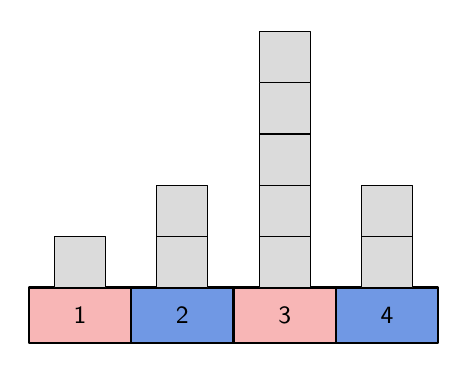
\begin{tikzpicture}[x=1mm,y=1mm,line join=round]
\path (0,0) rectangle (52,40.0);
\draw[thick, fill=slotred] (0,0) rectangle (13,7);
\node[font=\small] at (6.5,3.5) {1};
\draw[fill=black!14] (3.25,7.0) rectangle (9.75,13.5);
\draw[thick, fill=slotblue] (13,0) rectangle (26,7);
\node[font=\small] at (19.5,3.5) {2};
\draw[fill=black!14] (16.25,7.0) rectangle (22.75,13.5);
\draw[fill=black!14] (16.25,13.5) rectangle (22.75,20.0);
\draw[thick, fill=slotred] (26,0) rectangle (39,7);
\node[font=\small] at (32.5,3.5) {3};
\draw[fill=black!14] (29.25,7.0) rectangle (35.75,13.5);
\draw[fill=black!14] (29.25,13.5) rectangle (35.75,20.0);
\draw[fill=black!14] (29.25,20.0) rectangle (35.75,26.5);
\draw[fill=black!14] (29.25,26.5) rectangle (35.75,33.0);
\draw[fill=black!14] (29.25,33.0) rectangle (35.75,39.5);
\draw[thick, fill=slotblue] (39,0) rectangle (52,7);
\node[font=\small] at (45.5,3.5) {4};
\draw[fill=black!14] (42.25,7.0) rectangle (48.75,13.5);
\draw[fill=black!14] (42.25,13.5) rectangle (48.75,20.0);
\end{tikzpicture}\end{minipage}\hfill\begin{minipage}[b]{0.48\linewidth}\centering 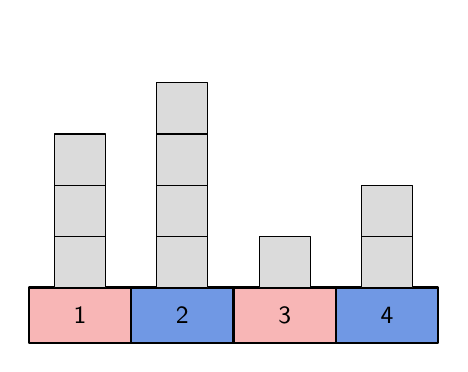
\begin{tikzpicture}[x=1mm,y=1mm,line join=round]
\path (0,0) rectangle (52,40.0);
\draw[thick, fill=slotred] (0,0) rectangle (13,7);
\node[font=\small] at (6.5,3.5) {1};
\draw[fill=black!14] (3.25,7.0) rectangle (9.75,13.5);
\draw[fill=black!14] (3.25,13.5) rectangle (9.75,20.0);
\draw[fill=black!14] (3.25,20.0) rectangle (9.75,26.5);
\draw[thick, fill=slotblue] (13,0) rectangle (26,7);
\node[font=\small] at (19.5,3.5) {2};
\draw[fill=black!14] (16.25,7.0) rectangle (22.75,13.5);
\draw[fill=black!14] (16.25,13.5) rectangle (22.75,20.0);
\draw[fill=black!14] (16.25,20.0) rectangle (22.75,26.5);
\draw[fill=black!14] (16.25,26.5) rectangle (22.75,33.0);
\draw[thick, fill=slotred] (26,0) rectangle (39,7);
\node[font=\small] at (32.5,3.5) {3};
\draw[fill=black!14] (29.25,7.0) rectangle (35.75,13.5);
\draw[thick, fill=slotblue] (39,0) rectangle (52,7);
\node[font=\small] at (45.5,3.5) {4};
\draw[fill=black!14] (42.25,7.0) rectangle (48.75,13.5);
\draw[fill=black!14] (42.25,13.5) rectangle (48.75,20.0);
\end{tikzpicture}\end{minipage}\par\vspace{14mm}
\noindent \begin{minipage}[b]{0.48\linewidth}\centering 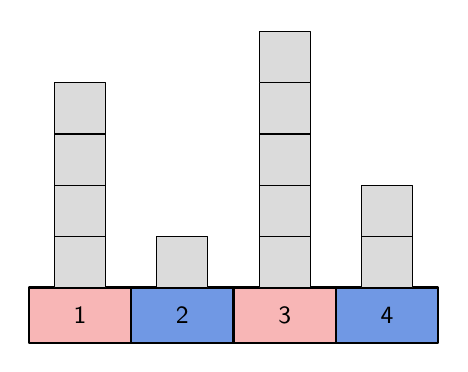
\begin{tikzpicture}[x=1mm,y=1mm,line join=round]
\path (0,0) rectangle (52,40.0);
\draw[thick, fill=slotred] (0,0) rectangle (13,7);
\node[font=\small] at (6.5,3.5) {1};
\draw[fill=black!14] (3.25,7.0) rectangle (9.75,13.5);
\draw[fill=black!14] (3.25,13.5) rectangle (9.75,20.0);
\draw[fill=black!14] (3.25,20.0) rectangle (9.75,26.5);
\draw[fill=black!14] (3.25,26.5) rectangle (9.75,33.0);
\draw[thick, fill=slotblue] (13,0) rectangle (26,7);
\node[font=\small] at (19.5,3.5) {2};
\draw[fill=black!14] (16.25,7.0) rectangle (22.75,13.5);
\draw[thick, fill=slotred] (26,0) rectangle (39,7);
\node[font=\small] at (32.5,3.5) {3};
\draw[fill=black!14] (29.25,7.0) rectangle (35.75,13.5);
\draw[fill=black!14] (29.25,13.5) rectangle (35.75,20.0);
\draw[fill=black!14] (29.25,20.0) rectangle (35.75,26.5);
\draw[fill=black!14] (29.25,26.5) rectangle (35.75,33.0);
\draw[fill=black!14] (29.25,33.0) rectangle (35.75,39.5);
\draw[thick, fill=slotblue] (39,0) rectangle (52,7);
\node[font=\small] at (45.5,3.5) {4};
\draw[fill=black!14] (42.25,7.0) rectangle (48.75,13.5);
\draw[fill=black!14] (42.25,13.5) rectangle (48.75,20.0);
\end{tikzpicture}\end{minipage}\hfill\begin{minipage}[b]{0.48\linewidth}\centering 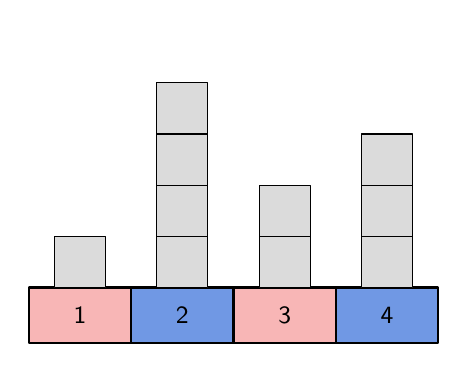
\begin{tikzpicture}[x=1mm,y=1mm,line join=round]
\path (0,0) rectangle (52,40.0);
\draw[thick, fill=slotred] (0,0) rectangle (13,7);
\node[font=\small] at (6.5,3.5) {1};
\draw[fill=black!14] (3.25,7.0) rectangle (9.75,13.5);
\draw[thick, fill=slotblue] (13,0) rectangle (26,7);
\node[font=\small] at (19.5,3.5) {2};
\draw[fill=black!14] (16.25,7.0) rectangle (22.75,13.5);
\draw[fill=black!14] (16.25,13.5) rectangle (22.75,20.0);
\draw[fill=black!14] (16.25,20.0) rectangle (22.75,26.5);
\draw[fill=black!14] (16.25,26.5) rectangle (22.75,33.0);
\draw[thick, fill=slotred] (26,0) rectangle (39,7);
\node[font=\small] at (32.5,3.5) {3};
\draw[fill=black!14] (29.25,7.0) rectangle (35.75,13.5);
\draw[fill=black!14] (29.25,13.5) rectangle (35.75,20.0);
\draw[thick, fill=slotblue] (39,0) rectangle (52,7);
\node[font=\small] at (45.5,3.5) {4};
\draw[fill=black!14] (42.25,7.0) rectangle (48.75,13.5);
\draw[fill=black!14] (42.25,13.5) rectangle (48.75,20.0);
\draw[fill=black!14] (42.25,20.0) rectangle (48.75,26.5);
\end{tikzpicture}\end{minipage}\par\vspace{14mm}\newpage\problem Now you go first on the colored strip. Can you play so that your partner can never beat you?\par\vspace{6mm}\noindent \begin{minipage}[b]{0.48\linewidth}\centering 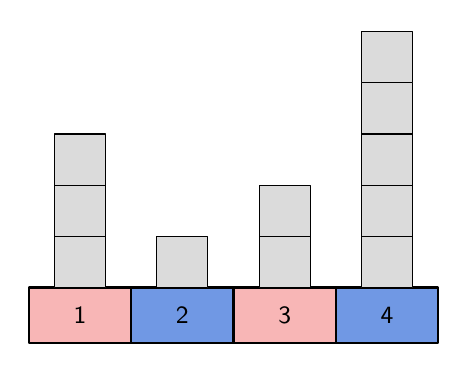
\begin{tikzpicture}[x=1mm,y=1mm,line join=round]
\path (0,0) rectangle (52,40.0);
\draw[thick, fill=slotred] (0,0) rectangle (13,7);
\node[font=\small] at (6.5,3.5) {1};
\draw[fill=black!14] (3.25,7.0) rectangle (9.75,13.5);
\draw[fill=black!14] (3.25,13.5) rectangle (9.75,20.0);
\draw[fill=black!14] (3.25,20.0) rectangle (9.75,26.5);
\draw[thick, fill=slotblue] (13,0) rectangle (26,7);
\node[font=\small] at (19.5,3.5) {2};
\draw[fill=black!14] (16.25,7.0) rectangle (22.75,13.5);
\draw[thick, fill=slotred] (26,0) rectangle (39,7);
\node[font=\small] at (32.5,3.5) {3};
\draw[fill=black!14] (29.25,7.0) rectangle (35.75,13.5);
\draw[fill=black!14] (29.25,13.5) rectangle (35.75,20.0);
\draw[thick, fill=slotblue] (39,0) rectangle (52,7);
\node[font=\small] at (45.5,3.5) {4};
\draw[fill=black!14] (42.25,7.0) rectangle (48.75,13.5);
\draw[fill=black!14] (42.25,13.5) rectangle (48.75,20.0);
\draw[fill=black!14] (42.25,20.0) rectangle (48.75,26.5);
\draw[fill=black!14] (42.25,26.5) rectangle (48.75,33.0);
\draw[fill=black!14] (42.25,33.0) rectangle (48.75,39.5);
\end{tikzpicture}\end{minipage}\hfill\begin{minipage}[b]{0.48\linewidth}\centering 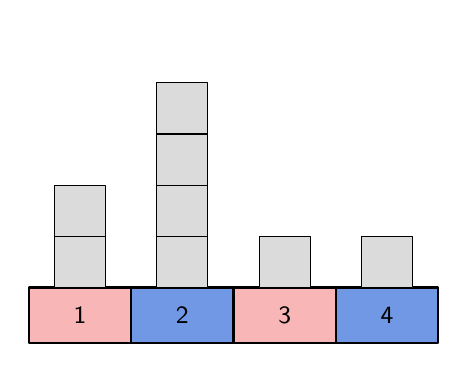
\begin{tikzpicture}[x=1mm,y=1mm,line join=round]
\path (0,0) rectangle (52,40.0);
\draw[thick, fill=slotred] (0,0) rectangle (13,7);
\node[font=\small] at (6.5,3.5) {1};
\draw[fill=black!14] (3.25,7.0) rectangle (9.75,13.5);
\draw[fill=black!14] (3.25,13.5) rectangle (9.75,20.0);
\draw[thick, fill=slotblue] (13,0) rectangle (26,7);
\node[font=\small] at (19.5,3.5) {2};
\draw[fill=black!14] (16.25,7.0) rectangle (22.75,13.5);
\draw[fill=black!14] (16.25,13.5) rectangle (22.75,20.0);
\draw[fill=black!14] (16.25,20.0) rectangle (22.75,26.5);
\draw[fill=black!14] (16.25,26.5) rectangle (22.75,33.0);
\draw[thick, fill=slotred] (26,0) rectangle (39,7);
\node[font=\small] at (32.5,3.5) {3};
\draw[fill=black!14] (29.25,7.0) rectangle (35.75,13.5);
\draw[thick, fill=slotblue] (39,0) rectangle (52,7);
\node[font=\small] at (45.5,3.5) {4};
\draw[fill=black!14] (42.25,7.0) rectangle (48.75,13.5);
\end{tikzpicture}\end{minipage}\par\vspace{10mm}\noindent \begin{minipage}[b]{0.49\linewidth}\centering 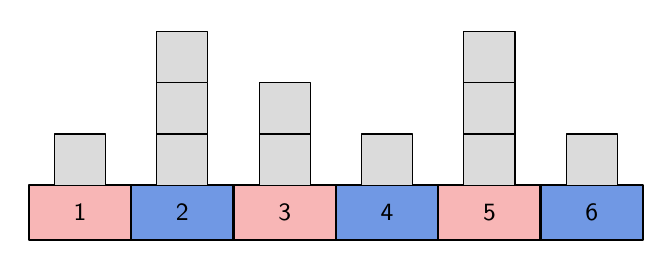
\begin{tikzpicture}[x=1mm,y=1mm,line join=round]
\path (0,0) rectangle (78,27.0);
\draw[thick, fill=slotred] (0,0) rectangle (13,7);
\node[font=\small] at (6.5,3.5) {1};
\draw[fill=black!14] (3.25,7.0) rectangle (9.75,13.5);
\draw[thick, fill=slotblue] (13,0) rectangle (26,7);
\node[font=\small] at (19.5,3.5) {2};
\draw[fill=black!14] (16.25,7.0) rectangle (22.75,13.5);
\draw[fill=black!14] (16.25,13.5) rectangle (22.75,20.0);
\draw[fill=black!14] (16.25,20.0) rectangle (22.75,26.5);
\draw[thick, fill=slotred] (26,0) rectangle (39,7);
\node[font=\small] at (32.5,3.5) {3};
\draw[fill=black!14] (29.25,7.0) rectangle (35.75,13.5);
\draw[fill=black!14] (29.25,13.5) rectangle (35.75,20.0);
\draw[thick, fill=slotblue] (39,0) rectangle (52,7);
\node[font=\small] at (45.5,3.5) {4};
\draw[fill=black!14] (42.25,7.0) rectangle (48.75,13.5);
\draw[thick, fill=slotred] (52,0) rectangle (65,7);
\node[font=\small] at (58.5,3.5) {5};
\draw[fill=black!14] (55.25,7.0) rectangle (61.75,13.5);
\draw[fill=black!14] (55.25,13.5) rectangle (61.75,20.0);
\draw[fill=black!14] (55.25,20.0) rectangle (61.75,26.5);
\draw[thick, fill=slotblue] (65,0) rectangle (78,7);
\node[font=\small] at (71.5,3.5) {6};
\draw[fill=black!14] (68.25,7.0) rectangle (74.75,13.5);
\end{tikzpicture}\end{minipage}\hfill\begin{minipage}[b]{0.49\linewidth}\centering 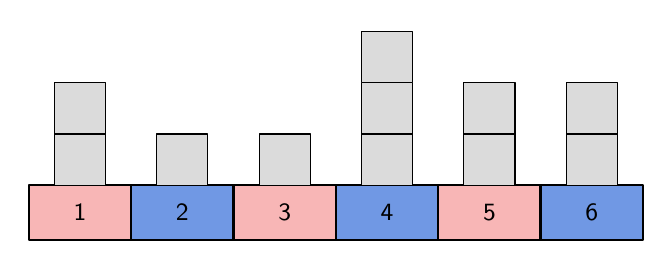
\begin{tikzpicture}[x=1mm,y=1mm,line join=round]
\path (0,0) rectangle (78,27.0);
\draw[thick, fill=slotred] (0,0) rectangle (13,7);
\node[font=\small] at (6.5,3.5) {1};
\draw[fill=black!14] (3.25,7.0) rectangle (9.75,13.5);
\draw[fill=black!14] (3.25,13.5) rectangle (9.75,20.0);
\draw[thick, fill=slotblue] (13,0) rectangle (26,7);
\node[font=\small] at (19.5,3.5) {2};
\draw[fill=black!14] (16.25,7.0) rectangle (22.75,13.5);
\draw[thick, fill=slotred] (26,0) rectangle (39,7);
\node[font=\small] at (32.5,3.5) {3};
\draw[fill=black!14] (29.25,7.0) rectangle (35.75,13.5);
\draw[thick, fill=slotblue] (39,0) rectangle (52,7);
\node[font=\small] at (45.5,3.5) {4};
\draw[fill=black!14] (42.25,7.0) rectangle (48.75,13.5);
\draw[fill=black!14] (42.25,13.5) rectangle (48.75,20.0);
\draw[fill=black!14] (42.25,20.0) rectangle (48.75,26.5);
\draw[thick, fill=slotred] (52,0) rectangle (65,7);
\node[font=\small] at (58.5,3.5) {5};
\draw[fill=black!14] (55.25,7.0) rectangle (61.75,13.5);
\draw[fill=black!14] (55.25,13.5) rectangle (61.75,20.0);
\draw[thick, fill=slotblue] (65,0) rectangle (78,7);
\node[font=\small] at (71.5,3.5) {6};
\draw[fill=black!14] (68.25,7.0) rectangle (74.75,13.5);
\draw[fill=black!14] (68.25,13.5) rectangle (74.75,20.0);
\end{tikzpicture}\end{minipage}\par\vspace{4mm}\problem You go first on these colored rows. Which rows can you win, however your partner plays? Ring them.\par\vspace{6mm}\noindent \begin{minipage}[b]{0.32\linewidth}\centering 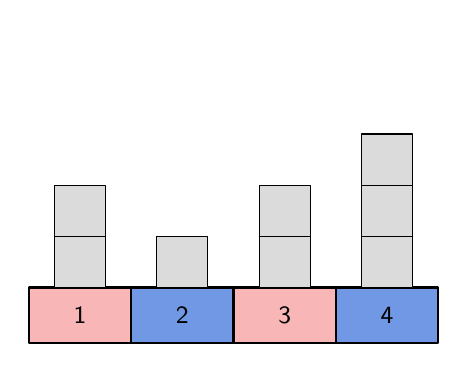
\begin{tikzpicture}[x=1mm,y=1mm,line join=round]
\path (0,0) rectangle (52,40.0);
\draw[thick, fill=slotred] (0,0) rectangle (13,7);
\node[font=\small] at (6.5,3.5) {1};
\draw[fill=black!14] (3.25,7.0) rectangle (9.75,13.5);
\draw[fill=black!14] (3.25,13.5) rectangle (9.75,20.0);
\draw[thick, fill=slotblue] (13,0) rectangle (26,7);
\node[font=\small] at (19.5,3.5) {2};
\draw[fill=black!14] (16.25,7.0) rectangle (22.75,13.5);
\draw[thick, fill=slotred] (26,0) rectangle (39,7);
\node[font=\small] at (32.5,3.5) {3};
\draw[fill=black!14] (29.25,7.0) rectangle (35.75,13.5);
\draw[fill=black!14] (29.25,13.5) rectangle (35.75,20.0);
\draw[thick, fill=slotblue] (39,0) rectangle (52,7);
\node[font=\small] at (45.5,3.5) {4};
\draw[fill=black!14] (42.25,7.0) rectangle (48.75,13.5);
\draw[fill=black!14] (42.25,13.5) rectangle (48.75,20.0);
\draw[fill=black!14] (42.25,20.0) rectangle (48.75,26.5);
\end{tikzpicture}\end{minipage}\hfill\begin{minipage}[b]{0.32\linewidth}\centering 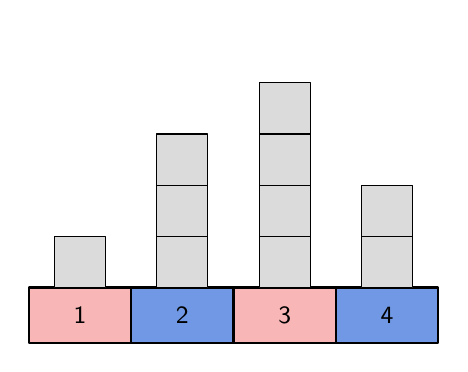
\begin{tikzpicture}[x=1mm,y=1mm,line join=round]
\path (0,0) rectangle (52,40.0);
\draw[thick, fill=slotred] (0,0) rectangle (13,7);
\node[font=\small] at (6.5,3.5) {1};
\draw[fill=black!14] (3.25,7.0) rectangle (9.75,13.5);
\draw[thick, fill=slotblue] (13,0) rectangle (26,7);
\node[font=\small] at (19.5,3.5) {2};
\draw[fill=black!14] (16.25,7.0) rectangle (22.75,13.5);
\draw[fill=black!14] (16.25,13.5) rectangle (22.75,20.0);
\draw[fill=black!14] (16.25,20.0) rectangle (22.75,26.5);
\draw[thick, fill=slotred] (26,0) rectangle (39,7);
\node[font=\small] at (32.5,3.5) {3};
\draw[fill=black!14] (29.25,7.0) rectangle (35.75,13.5);
\draw[fill=black!14] (29.25,13.5) rectangle (35.75,20.0);
\draw[fill=black!14] (29.25,20.0) rectangle (35.75,26.5);
\draw[fill=black!14] (29.25,26.5) rectangle (35.75,33.0);
\draw[thick, fill=slotblue] (39,0) rectangle (52,7);
\node[font=\small] at (45.5,3.5) {4};
\draw[fill=black!14] (42.25,7.0) rectangle (48.75,13.5);
\draw[fill=black!14] (42.25,13.5) rectangle (48.75,20.0);
\end{tikzpicture}\end{minipage}\hfill\begin{minipage}[b]{0.32\linewidth}\centering 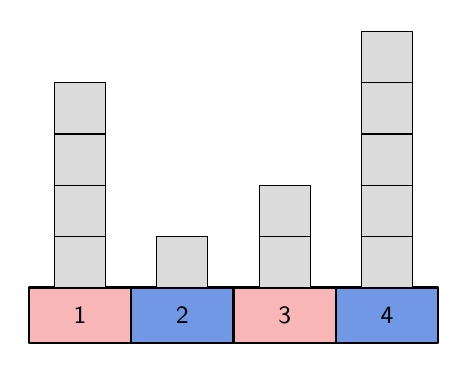
\begin{tikzpicture}[x=1mm,y=1mm,line join=round]
\path (0,0) rectangle (52,40.0);
\draw[thick, fill=slotred] (0,0) rectangle (13,7);
\node[font=\small] at (6.5,3.5) {1};
\draw[fill=black!14] (3.25,7.0) rectangle (9.75,13.5);
\draw[fill=black!14] (3.25,13.5) rectangle (9.75,20.0);
\draw[fill=black!14] (3.25,20.0) rectangle (9.75,26.5);
\draw[fill=black!14] (3.25,26.5) rectangle (9.75,33.0);
\draw[thick, fill=slotblue] (13,0) rectangle (26,7);
\node[font=\small] at (19.5,3.5) {2};
\draw[fill=black!14] (16.25,7.0) rectangle (22.75,13.5);
\draw[thick, fill=slotred] (26,0) rectangle (39,7);
\node[font=\small] at (32.5,3.5) {3};
\draw[fill=black!14] (29.25,7.0) rectangle (35.75,13.5);
\draw[fill=black!14] (29.25,13.5) rectangle (35.75,20.0);
\draw[thick, fill=slotblue] (39,0) rectangle (52,7);
\node[font=\small] at (45.5,3.5) {4};
\draw[fill=black!14] (42.25,7.0) rectangle (48.75,13.5);
\draw[fill=black!14] (42.25,13.5) rectangle (48.75,20.0);
\draw[fill=black!14] (42.25,20.0) rectangle (48.75,26.5);
\draw[fill=black!14] (42.25,26.5) rectangle (48.75,33.0);
\draw[fill=black!14] (42.25,33.0) rectangle (48.75,39.5);
\end{tikzpicture}\end{minipage}\par\vspace{2mm}
\end{document}
